\documentclass[11pt,a4paper]{article}
\usepackage[utf8]{inputenc}
\usepackage[french]{babel}
\usepackage[T1]{fontenc}

\usepackage{amsmath}
\usepackage{amsfonts}
\usepackage{amssymb}

\newcommand{\NomAuteur}{Fabrice BOISSIER}
\newcommand{\TitreMatiere}{Architecture des Ordinateurs}
\newcommand{\NomUniv}{EPITA - Bachelor Cyber Sécurité}
\newcommand{\NiveauUniv}{CYBER1}
\newcommand{\NumGroupe}{CYBER1}
\newcommand{\AnneeUniv}{2023-2024}
\newcommand{\DateExam}{décembre 2023}
\newcommand{\TypeExam}{CORRECTION Partiel}
\newcommand{\TitreExam}{\TitreMatiere}
\newcommand{\DureeExam}{2h00}
\newcommand{\MyWaterMark}{\AnneeUniv} % Watermark de protection

% Ajout de mes classes & definitions
\usepackage{MetalExam} % Appelle un .sty

% "Tableau" et pas "Table"
\addto\captionsfrench{\def\tablename{Tableau}}

%%%%%%%%%%%%%%%%%%%%%%%
%Header
%%%%%%%%%%%%%%%%%%%%%%%
\lhead{\TypeExam}							%Gauche Haut
\chead{\NomUniv}							%Centre Haut
\rhead{\NumGroupe}							%Droite Haut
\lfoot{\DateExam}							%Gauche Bas
\cfoot{\thepage{} / \pageref*{LastPage}}	%Centre Bas
\rfoot{\texttt{\TitreMatiere}}				%Droite Bas

%%%%%

\usepackage{tabularx}

\newlength{\LabelWidth}%
%\setlength{\LabelWidth}{1.3in}%
\setlength{\LabelWidth}{1cm}%
%\settowidth{\LabelWidth}{Employee E-mail:}%  Specify the widest text here.

% Optional first parameter here specifies the alignment of
% the text within the \makebox.  Default is [l] for left
% alignment. Other options are [r] and [c] for right and center
\newcommand*{\AdjustSize}[2][l]{\makebox[\LabelWidth][#1]{#2}}%


\definecolor{mGreen}{rgb}{0,0.6,0}
\definecolor{mGray}{rgb}{0.5,0.5,0.5}
\definecolor{mPurple}{rgb}{0.58,0,0.82}
\definecolor{backgroundColour}{rgb}{0.95,0.95,0.92}

\lstdefinestyle{CStyle}{
    backgroundcolor=\color{backgroundColour},
    commentstyle=\color{mGreen},
    keywordstyle=\color{magenta},
    numberstyle=\tiny\color{mGray},
    stringstyle=\color{mPurple},
    basicstyle=\footnotesize,
    breakatwhitespace=false,
    breaklines=true,
    captionpos=b,
    keepspaces=true,
    numbers=left,
    numbersep=5pt,
    showspaces=false,
    showstringspaces=false,
    showtabs=false,
    tabsize=2,
    language=C
}


\hyphenation{op-tical net-works SIGKILL}


\begin{document}

%\MakeExamTitleDuree     % Pour afficher la duree
\MakeExamTitle                   % Ne pas afficher la duree

%% \MakeStudentName    %% A reutiliser sur chaque nouvelle page

\bigskip
%\bigskip

Vous devez respecter les consignes suivantes, sous peine de 0 :

\begin{itemize}
\item Lisez le sujet en entier avec attention
\item Répondez sur le sujet
\item Ne détachez pas les agrafes du sujet
\item \'Ecrivez lisiblement vos réponses (si nécessaire en majuscules)
\item Les appareils électroniques sont tous interdits (calculatrices également)
\item Ne trichez pas
\end{itemize}

%\bigskip

\vfillFirst

% Conversions binaires
\section{Conversions Binaires (6 points)}

\subsection{(1 point) Rappelez les 14 premières puissances de 2 : }

\bigskip

%\begin{table}[ht!]
\centerline{
\begin{tabular}{ | m{0.5cm} | m{0.5cm} | m{0.5cm} | m{0.5cm} | m{0.65cm} | m{0.65cm} | m{0.65cm} | m{1cm} | m{1cm} | m{1cm} | m{1.5cm} | m{1.5cm} | m{1.5cm} | m{1.5cm} |}
\hline
$ 2^{0} $ & $ 2^{1} $ & $ 2^{2} $ & $ 2^{3} $ & $ 2^{4} $ & $ 2^{5} $ & $ 2^{6} $ & $ 2^{7} $ & $ 2^{8} $ & $ 2^{9} $ & $ 2^{10} $ & $ 2^{11} $ &  $ 2^{12} $ &  $ 2^{13} $ \\
\hline
 & & & & & & & & & & & & & \\
 1 & 2 & 4 & 8 & 16 & 32 & 64 & 128 & 256 & 512 & 1024 & 2048 & 4096 & 8192 \\
 & & & & & & & & & & & & & \\
\hline
\end{tabular}
}
%\end{table}

\bigskip
\bigskip

\subsection{(2 points) Convertissez ces nombres en décimaux : }

\bigskip

%\begin{table}[ht!]
\centerline{
\begin{tabular}{ c |  m{2cm}   c   m{2cm} | m{2cm}   c   m{2cm} }
 & & & &  & & \\
                                & & non-signé & & & signé & \\
 & & & &  & & \\
\hline
 & & & &  & & \\
$ \% \, 1010 \; 0011 \; 1011 $  & &  2619  & & &  -1477  & \\
 & & & &  & & \\
\hline
 & & & &  & & \\
\$ B52                          & &  2898  & & &  -1198  & \\
 & & & &  & & \\
\end{tabular}
}
%\end{table}

\bigskip
\bigskip

\subsection{(3 points) Convertissez ces nombres décimaux en binaire sur 12 bits, puis en hexadécimal.}

\bigskip

%\centerline{
%\begin{tabular}{ c |  m{2cm}   c   m{2cm} | m{2cm}   c   m{2cm} }
%                                & & binaire & & & hexadécimal & \\
% & & & &  & & \\
%\hline
% & & & &  & & \\
%$ 42 $    & &           & & &  & \\
% & & & &  & & \\
%\hline
%% & & & &  & & \\
%%$ 1664 $  & &           & & &  & \\
%% & & & &  & & \\
%%\hline
% & & & &  & & \\
%$ 2051 $  & &           & & &  & \\
% & & & &  & & \\
%\hline
% & & & &  & & \\
%$ -218 $  & &           & & &  & \\
% & & & &  & & \\
%\end{tabular}
%}


%\begin{table}[ht!]
\centerline{
\begin{tabular}{ | c |C{0.33cm}||C{0.33cm}|C{0.33cm}|C{0.33cm}|C{0.33cm}||C{0.33cm}|C{0.33cm}|C{0.33cm}|C{0.33cm}||C{0.33cm}|C{0.33cm}|C{0.33cm}|C{0.33cm}| c |}
\hline
                         & \multicolumn{13}{c|}{binaire} & \multicolumn{1}{c|}{hexadécimal} \\
%                         & \multicolumn{12}{c|}{binaire} & \multicolumn{1}{c|}{hexadécimal} \\
\hline

\multirow[c]{2}{*}[0in]{42}   & \cellcolor{black!15}     & & & & & & & & & & & &    & \\
                              & \cellcolor{black!15} \%  & 0 & 0 & 0 & 0 & 0 & 0 & 1 & 0 & 1 & 0 & 1 & 0 & \$ 02A \\
\hline

\multirow[c]{2}{*}[0in]{1789} & \cellcolor{black!15}     & & & & & & & & & & & &    & \\
                              & \cellcolor{black!15} \%  & 0 & 1 & 1 & 0 & 1 & 1 & 1 & 1 & 1 & 1 & 0 & 1 & \$ 6FD \\
\hline
\multirow[c]{2}{*}[0in]{-404} & \cellcolor{black!15}     & & & & & & & & & & & &    & \\
                              & \cellcolor{black!15} \%  & 1 & 1 & 1 & 0 & 0 & 1 & 1 & 0 & 1 & 1 & 0 & 0 & \$ E6C \\
\hline
%\multirow[c]{2}{*}[0in]{2051} & \multicolumn{6}{c|}{ } & \multicolumn{6}{c|}{ } \\
%                              & \multicolumn{6}{c|}{ } & \multicolumn{6}{c|}{ } \\
%                              & \multicolumn{6}{c|}{ } & \multicolumn{6}{c|}{ } \\
%\hline
\end{tabular}
}
%\end{table}

\vfillLast

%\bigskip


%\vfillFirst
%
%\begin{center}
%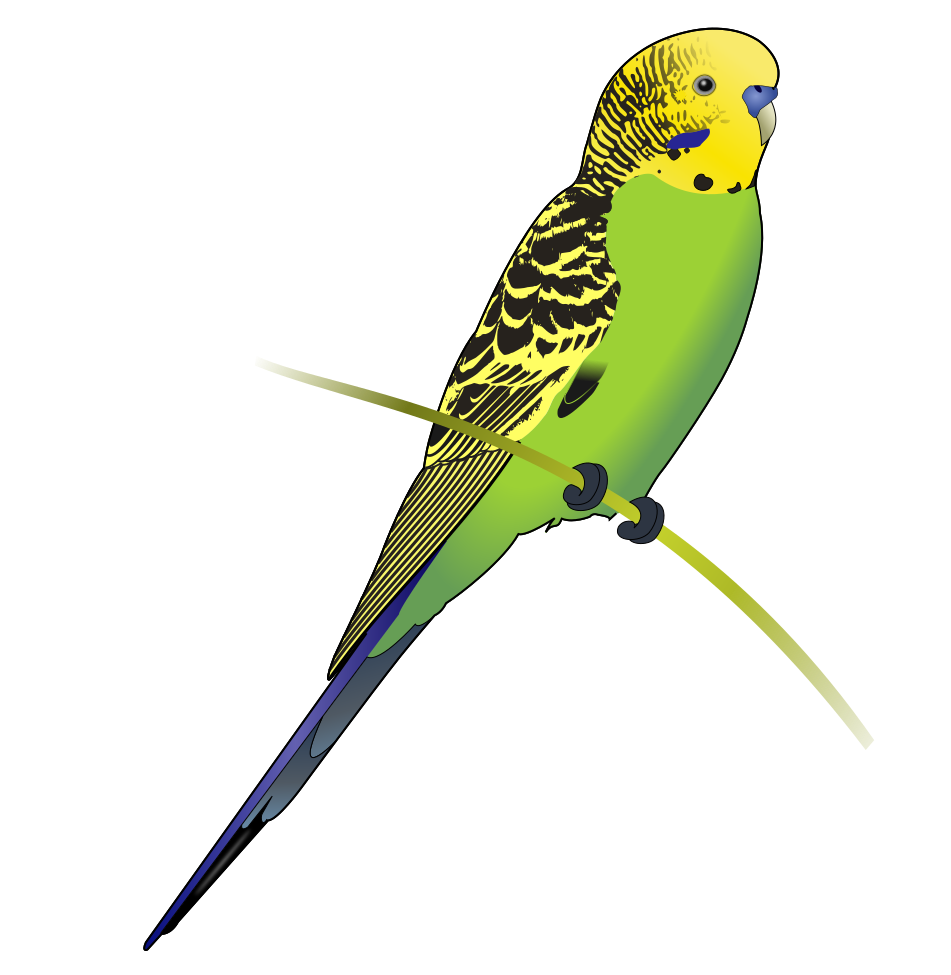
\includegraphics[scale=0.2]{img/others/Budgerigar_diagram.png}
%\end{center}
%
%\vfillLast

\clearpage

%%%%%%%%%%%%%%%%%%%%%%%%%%%%%%%%%%%%%%%%%%%%%%%%%%%%%%%
%%%%%%%%%%%%%%%%%%%%%%%%%%%%%%%%%%%%%%%%%%%%%%%%%%%%%%%
%%%%%%%%%%%%%%%%%%%%%%%%%%%%%%%%%%%%%%%%%%%%%%%%%%%%%%%

% Conversions flottants
\section{Conversions Flottants (3 points)}

\subsection{(1 point) Rappelez les formats IEEE 754 des flottants, les formules décimales associées, et les biais : }

\bigskip

\begin{center}
\begin{tabular}{c | C{2cm} | C{2.5cm} | C{3cm} }
 & & & \\
précision & Signe & Exposant & Mantisse \\
 & & & \\
\hline
 & & & \\
simple précision (32 bits) & 1 & 8 & 23 \\
 & & & \\
\hline
 & & & \\
double précision (64 bits) & 1 & 11 & 52 \\
 & & & \\
\end{tabular}
\end{center}

\bigskip

\begin{table}[!ht]
  \centering
  \begin{minipage}{0.40\textwidth}
    \centering

\begin{tabular}{| c | C{1.5cm} |}
\hline
 & \\
 & biais \\
 & \\
\hline
 & \\
simple précision & 127 \\
 & \\
\hline
 & \\
double précision & 1023 \\
 & \\
\hline
\end{tabular}

  \end{minipage}
  \hfillx
  \begin{minipage}{0.60\textwidth}
    \centering

Formule(s) mathématique(s) simple précision :

\medskip

normalisés : $ (-1)^{signe} \times 2^{exposant - biais} \times (1 + mantisse) $

\smallskip

dénormalisés : $ (-1)^{signe} \times 2^{1 - biais} \times (0 + mantisse) $


\vspace*{0.75cm}


Formule(s) mathématique(s) double précision :

normalisés : $ (-1)^{signe} \times 2^{exposant - biais} \times (1 + mantisse) $

\smallskip

dénormalisés : $ (-1)^{signe} \times 2^{1 - biais} \times (0 + mantisse) $

\vspace*{1.75cm}

  \end{minipage}
\end{table}


%\bigskip
\vspace*{-0.5cm}

\subsection{(2 points) Calculez la valeur décimale du plus petit flottant dénormalisé en double précision : }

\bigskip

\bigskip

\begin{tabular}{l c l}
Exposant (11 bits) :  & $ 000 \; 0000 \; 0000_{2} $ & Exposant nul (dénormalisé)\\
Mantisse (52 bits) : & $ 0 \; 0000 \; 0000 \; 0001_{16} $ & \\
\end{tabular}

\bigskip

\begin{center}
$ (-1)^{\text{signe}} \times \text{mantisse} \times 2^{\text{1 - biais}} $

\smallskip
$ = $
\smallskip

$ (-1)^{\text{0}} \times 2^{-52} \times 2^{1 - 1023} $

\smallskip
$ = $
\smallskip

$ 2^{-52} \times 2^{-1022} $

\smallskip
$ = $
\smallskip

$ 2^{-1074} $
\end{center}

Le plus petit nombre positif non-nul dénormalisé en simple précision est donc $ 2^{-1074} $.

\clearpage

%%%%%%%%%%%%%%%%%%%%%%%%%%%%%%%%%%%%%%%%%%%%%%%%%%%%%%%
%%%%%%%%%%%%%%%%%%%%%%%%%%%%%%%%%%%%%%%%%%%%%%%%%%%%%%%
%%%%%%%%%%%%%%%%%%%%%%%%%%%%%%%%%%%%%%%%%%%%%%%%%%%%%%%

% Conversions dans tous les formats
\section{Interprétations (6 points)}

\subsection{(6 points) Convertissez la donnée suivante selon chaque interprétation : }

\bigskip

\begin{center}
\textbf{\Large \$ 4231 2000 }
\end{center}

%\medskip
\smallskip

\begin{table}[!ht]
  \centering
  \begin{minipage}{0.50\textwidth}
    \centering

Un flottant simple précision
% 44.28125

\medskip

\begin{tabular}{| C{5cm} |}
\hline
\phantom{42} \\
$ 44,28125 $  $\;\; = \; \;$  $ 1417 \times 2^{-5} $ \\
\phantom{42} \\
\hline
\end{tabular}

  \end{minipage}
  \hfillx
  \begin{minipage}{0.50\textwidth}
    \centering

Quatre caractères
% 'B'   '1'   ' '   '\0'

\medskip

\begin{tabular}{| C{1cm} | C{1cm} | C{1cm} | C{1cm} |}
\hline
\phantom{I} & \phantom{I} & \phantom{I} & \phantom{I} \\
'B' & '1' & ' $\,$ ' & '\textbackslash{}0' \\
\phantom{I} & \phantom{I} & {\footnotesize \textit{(espace)}} & \phantom{I} \\
\hline
\end{tabular}

  \end{minipage}
\end{table}

\smallskip

\begin{table}[!ht]
  \centering
  \begin{minipage}{0.50\textwidth}
    \centering

Deux entiers non signés en base 10

\medskip

\begin{tabular}{| C{3cm} | C{3cm} |}
\hline
\phantom{42} & \phantom{42} \\
16945 & 8192 \\
\phantom{42} & \phantom{42} \\
\hline
\end{tabular}

  \end{minipage}
  \hfillx
  \begin{minipage}{0.50\textwidth}
    \centering

Deux entiers signés en base 10

\medskip

\begin{tabular}{| C{3cm} | C{3cm} |}
\hline
\phantom{42} & \phantom{42} \\
16945 & 8192 \\
\phantom{42} & \phantom{42} \\
\hline
\end{tabular}

  \end{minipage}
\end{table}

\smallskip

\begin{table}[!ht]
  \centering
  \begin{minipage}{0.50\textwidth}
    \centering

Deux entiers base 10 depuis le code Gray

\medskip

\begin{tabular}{| C{3cm} | C{3cm} |}
\hline
\phantom{42} & \phantom{42} \\
32193 & 16383 \\
\phantom{42} & \phantom{42} \\
\hline
\end{tabular}

  \end{minipage}
  \hfillx
  \begin{minipage}{0.50\textwidth}
    \centering

Deux entiers base 10 depuis le BCD

\medskip

\begin{tabular}{| C{3cm} | C{3cm} |}
\hline
\phantom{42} & \phantom{42} \\
4231 & 2000 \\
\phantom{42} & \phantom{42} \\
\hline
\end{tabular}

  \end{minipage}
\end{table}

\bigskip

%\clearpage

%%%%%%%%%%%%%%%%%%%%%%%%%%%%%%%%%%%%%%%%%%%%%%%%%%%%%%%
%%%%%%%%%%%%%%%%%%%%%%%%%%%%%%%%%%%%%%%%%%%%%%%%%%%%%%%
%%%%%%%%%%%%%%%%%%%%%%%%%%%%%%%%%%%%%%%%%%%%%%%%%%%%%%%

% Circuits logiques
\section{Circuits logiques (5 points)}

\subsection{(1 point) \'Ecrivez la formule associée à ce schéma : }

%\bigskip
%\medskip
\smallskip

\begin{figure}[ht!]
\centering{
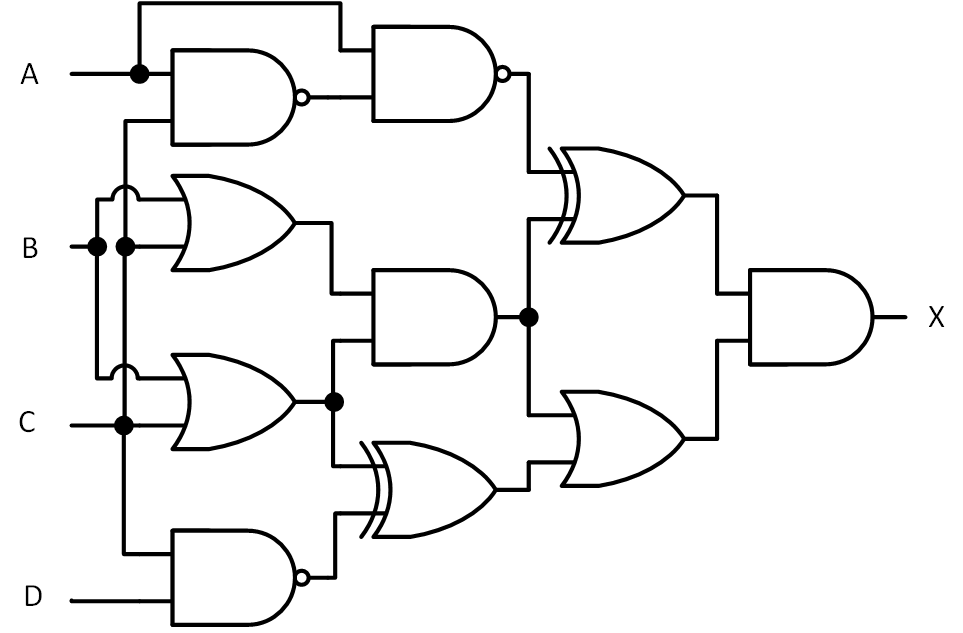
\includegraphics[scale=2]{./img/circuit_logique_1.png}
}
\end{figure}

\vspace*{-0.5cm}

%$ X = ((A NON-ET (A NON-ET C)) XOR ((B OU C) ET (B OU C))) ET (((B OU C) ET (B OU C)) OU ((B OU C) XOR (C NON-ET D))) $

\begin{equation*}
    \begin{split}
X = & ((a \; \text{NON-ET} \; (a \; \text{NON-ET} \; c)) \; \; \; \text{XOR} \; \; \; ((b \; \text{OU} \; c) \; \text{ET} \; (b \; \text{OU} \; c))) \\
    &   \; \; \; \; \; \; \text{ET} \\
    & (((b \; \text{OU} \; c) \; \text{ET} \; (b \; \text{OU} \; c)) \; \; \; \text{OU} \; \; \; ((b \; \text{OU} \; c) \; \text{XOR} \; (c \; \text{NON-ET} \; d)))\\
    \end{split}
\end{equation*}

$ X = (\overline{(A \cdot \overline{(A \cdot C)})} \oplus ((B + C) \cdot (B + C))) \cdot (((B + C) \cdot (B + C)) + ((B + C) \oplus \overline{(C \cdot D)})) $

%\bigskip
\clearpage


\begin{table}[!ht]
  \centering
  \begin{minipage}{0.50\textwidth}
    \centering

\subsection{(1 point) Remplissez la table de vérité de la formule précédente : }

\bigskip

\begin{center}
\begin{tabular}{|c|c|c|c||c|}
\hline
\cellcolor{black!15} \textbf{A} & \cellcolor{black!15} \textbf{B} & \cellcolor{black!15} \textbf{C} & \cellcolor{black!15} \textbf{D}  &  \cellcolor{black!15} \textbf{X} \\
\hline
\hline
0 & 0 & 0 & 0  &  \cellcolor{black!15} 1 \\ \hline
0 & 0 & 0 & 1  &  \cellcolor{black!15} 1 \\ \hline
0 & 0 & 1 & 0  &  \cellcolor{black!15} 0 \\ \hline
0 & 0 & 1 & 1  &  \cellcolor{black!15} 0 \\ \hline
0 & 1 & 0 & 0  &  \cellcolor{black!15} 0 \\ \hline
0 & 1 & 0 & 1  &  \cellcolor{black!15} 0 \\ \hline
0 & 1 & 1 & 0  &  \cellcolor{black!15} 0 \\ \hline
0 & 1 & 1 & 1  &  \cellcolor{black!15} 0 \\ \hline
1 & 0 & 0 & 0  &  \cellcolor{black!15} 0 \\ \hline
1 & 0 & 0 & 1  &  \cellcolor{black!15} 0 \\ \hline
1 & 0 & 1 & 0  &  \cellcolor{black!15} 0 \\ \hline
1 & 0 & 1 & 1  &  \cellcolor{black!15} 0 \\ \hline
1 & 1 & 0 & 0  &  \cellcolor{black!15} 1 \\ \hline
1 & 1 & 0 & 1  &  \cellcolor{black!15} 1 \\ \hline
1 & 1 & 1 & 0  &  \cellcolor{black!15} 0 \\ \hline
1 & 1 & 1 & 1  &  \cellcolor{black!15} 0 \\ \hline
\end{tabular}
\end{center}

  \end{minipage}
  \hfillx
  \begin{minipage}{0.50\textwidth}
%    \centering

\subsection{(2 points) Déduisez-en la formule des mintermes, ainsi que la formule des maxtermes : }

\bigskip

Mintermes :

%%%\vspace*{3.35cm}
%%\vspace*{7.22cm}
%\vspace*{3cm}

\begin{equation*}
    \begin{split}
X = & ( \overline{A} \cdot \overline{B} \cdot \overline{C} \cdot \overline{D} ) \; + \; ( \overline{A} \cdot \overline{B} \cdot \overline{C} \cdot D ) \; + \; \\
    & ( A \cdot B \cdot \overline{C} \cdot \overline{D} ) \; + \; ( A \cdot B \cdot \overline{C} \cdot D )
    \end{split}
\end{equation*}

\bigskip

Maxtermes :

%%%\vspace*{3.35cm}
%%\vspace*{7.22cm}
%\vspace*{11.44cm}

\begin{equation*}
    \begin{split}
X = & ( A + B + \overline{C} + D ) \; \cdot \; ( A + B + \overline{C} + \overline{D} ) \; \cdot \; \\
    & ( A + \overline{B} + C + D ) \; \cdot \; ( A + \overline{B} + C + \overline{D} ) \; \cdot \; \\
    & ( A + \overline{B} + \overline{C} + D ) \; \cdot \; ( A + \overline{B} + \overline{C} + \overline{D} ) \; \cdot \; \\
    & ( \overline{A} + B + C + D ) \; \cdot \; ( \overline{A} + B + C + \overline{D} ) \; \cdot \; \\
    & ( \overline{A} + B + \overline{C} + D ) \; \cdot \; ( \overline{A} + B + \overline{C} + \overline{D} ) \; \cdot \; \\
    & ( \overline{A} + \overline{B} + \overline{C} + D ) \; \cdot \; ( \overline{A} + \overline{B} + \overline{C} + \overline{D} )
    \end{split}
\end{equation*}

  \end{minipage}
\end{table}

\bigskip
%\vspace*{-0.5cm}

\subsection{(1 point) Remplissez le tableau de Karnaugh, formez les groupes, et déduisez-en la formule réduite : }

%\bigskip

\begin{table}[!ht]
  \centering
  \begin{minipage}{0.08\textwidth}
    \centering

\vfillFirst

AB

\vfillLast

  \end{minipage}
  \hfillx
  \begin{minipage}{0.37\textwidth}
    \centering

\begin{center}

CD

\medskip

\begin{tabular}{|C{0.75cm} || C{0.75cm}|C{0.75cm}|C{0.75cm}|C{0.75cm}|}
\hline
\cellcolor{black!65} & \cellcolor{black!15} 00 & \cellcolor{black!15} 01 & \cellcolor{black!15} 11 & \cellcolor{black!15} 10 \\
\hline
\hline
 \cellcolor{black!15} 00 &  \tikzmarknode{g1A}{1} & \tikzmarknode{g1B}{1} & 0 & 0 \\ \hline
 \cellcolor{black!15} 01 &  0 & 0 & 0 & 0 \\ \hline
 \cellcolor{black!15} 11 &  \tikzmarknode{g2A}{1} & \tikzmarknode{g2B}{1} & 0 & 0 \\ \hline
 \cellcolor{black!15} 10 &  0 & 0 & 0 & 0 \\ \hline
\end{tabular}

\tikz[remember picture, overlay]{
%%  \node[draw, rounded rectangle, fit=(g1A.center) (g1B.center)] {};
%%  \node[draw, rounded rectangle, fit=(g2A.center) (g2B.center)] {};
%  \node[draw, rounded rectangle, inner sep=3pt, minimum size=3mm, fit=(g1A.west) (g1B.east)] {};
%  \node[draw, rounded rectangle, inner sep=3pt, minimum size=3mm, fit=(g2A.west) (g2B.east)] {};

\tikzstyle{surround} = [thick, draw=red, rounded corners=1mm]
            \begin{pgfonlayer}{background}
                %This is working well with: scale = 1 / 0.4 = 2.5
                \node[surround, scale=1] (background) [fit = (g1A.north west) (g1B.south east) (g1A.north east) ] {};
%                \node[surround, scale=1] (background) [fit = (g2A.north west) (g2B.south east) (g2A.north east) ] {};
            \end{pgfonlayer}

\tikzstyle{surround} = [thick, draw=blue, rounded corners=1mm]
            \begin{pgfonlayer}{background}
                %This is working well with: scale = 1 / 0.4 = 2.5
%                \node[surround, scale=1] (background) [fit = (g1A.north west) (g1B.south east) (g1A.north east) ] {};
                \node[surround, scale=1] (background) [fit = (g2A.north west) (g2B.south east) (g2A.north east) ] {};
            \end{pgfonlayer}
}

\end{center}

  \end{minipage}
  \hfillx
  \begin{minipage}{0.55\textwidth}
    \centering

\vfillFirst

$ X = ( \overline{A} \cdot \overline{B} \cdot \overline{C} ) \; + \; ( A \cdot B \cdot \overline{C} ) $

\bigskip

$ X = ( \overline{A} \oplus \overline{B} ) \; \cdot \; \overline{C} $

\vfillLast

  \end{minipage}
\end{table}

%%%%%%%%%%%%%%%%%%%%%%%%%%%%%%%%%%%%%%%%%%%%%%%%%%%%%%%%%%%%%%%%%%%%%%%%%%%%%

%\vfillFirst
%
%\begin{center}
%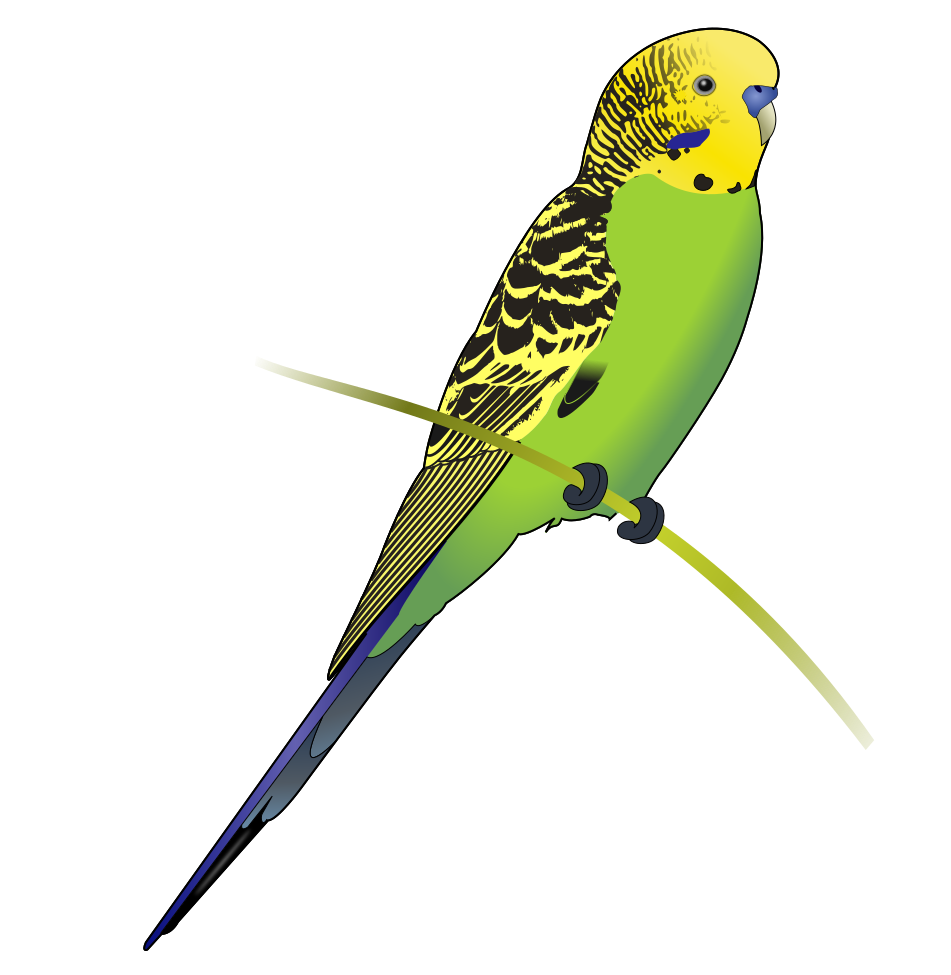
\includegraphics[scale=0.2]{img/others/Budgerigar_diagram.png}
%\end{center}
%
%\vfillLast

%\clearpage

%
%%\thispagestyle{empty}
%
%\vfillFirst
%
%\begin{center}
%
%\begin{LARGE}
%\textbf{SUJET}
%
%\bigskip
%
%\textbf{\MakeUppercase{\TitreMatiere}}
%\end{LARGE}
%
%\end{center}
%
%\vfillLast

\end{document}
